\documentclass[12pt]{article}
\usepackage[margin=1in]{geometry}
\usepackage{hyperref}

\bibliographystyle{apalike}

\usepackage{graphicx}

\title{Towards Benchmark Classification for GC Tuning}

\author{Olivier Fl\"uckiger}

\date{\today}

\begin{document}

\maketitle

\abstract

There are many GC algorithms described in the literature and used in practice.
However, an often overlooked detail are the heuristics, that all of them need to rely on.
When to grow the heap? How aggressively to shrink it again? Trigger a GC cycle early?
There are many knobs to turn, but a distinct lack of principled advice on how to do so.
In this article we propose a methodology for clustering programs by similar behavior, from the point of view of the GC.
We find that this method succeeds at identifying similarly behaving programs, but as such is not strong enough to predict the performance of a certain choice of parameters.

\vspace{2mm}
\section{Introduction}
A typical GC implementation has several tuneable parameters, such as heap grow rate, various thresholds for triggering collection cycles, and so on.
Picking an optimal set of parameters is a multi-dimensional optimization problem, and the resulting default parameters are always a compromise.
To better understand GC tuning, we propose to develop a methodology for classifying benchmarks (also called mutators) according to their behavior under varying GC parameters.

There are several applications of such a classification.
For a fair and unbiased comparison, we want to ensure, that we covered all facets of a GC algorithm.
For efficient testing, we might want to run the programs with the most nuanced behaviors first.
Also, we can provide more insightful evaluations, if we report performance numbers for each class.
Finally, if we know which classes of programs exist, we can detect them and adjust tuning parameters at runtime, overcoming the one size fits all nature of ahead-of-time GC tuning.

To cluster mutators we proceed in two steps.
First, we idealize their response to changing GC heuristics, by fitting an SVM model.
Second, we automatically cluster the generated models.

All the presented results in this article are based on the latest version of the reference R bytecode interpreter~\cite{r} and a standard R benchmark suite called \emph{rbench}\footnote{https://github.com/rbenchmark/benchmarks}.
The R GC uses a traditional treadmill~\cite{baker1992treadmill} design. We can't say how the results would generalize to other algorithms.
Source code and raw data can be found at\footnote{https://github.com/o-/ml\_hw/tree/master/project}.

\section{Technical Approach}

This section describes our data gathering, the preprocessing and the clustering approach.
As a first step, we gather benchmark execution times over a grid of GC parameter values.
In this experiment we looked at the following set of parameters: 

\begin{description}
  \item[R\_NGrowFrac] The occupancy percentage trigger value for heap growth.
  \item[R\_NGrowIncrFrac] The heap growth factor.
  \item[R\_MinFreeFrac] The trigger value for an old generation collection cycle.
  \item[R\_MaxKeepFrac] How many empty pages to retain.
\end{description}

The benchmarks where executed on a Lenovo X220 machine with an Intel Core i7-3520M CPU with a clock cycle of 2.90GHz and 16Gb of RAM running Fedora Linux version 27.
For each benchmark we identified the fastest execution time. We define a run to be \emph{fast} if it is within 3\% of the fastest one and \emph{slow} otherwise.
Thus our input data looks as follows:

\bigskip
\begin{tabular}{l l l l l l l}
  Program, & $P_1$, & $P_2$, & \dots, & $P_n$, & Time, & Slow/Fast \\
\end{tabular}
\bigskip

Then we train an SVM classifier, to predict \emph{fast} vs. \emph{slow} for a given set of GC parameters.
We use the SVM classifier by \cite{chang2011libsvm} from the \emph{e1071} R package with a radial basis kernel.
Hyperparameter selection is done by autotuning using gridsearch with 10-fold cross validation.
As an example see the preprocessing for the binary trees benchmark in \autoref{fig:bt}. 
Several benchmarks are not sensitive to changing GC parameters, since, for example, they do not allocate a significant number of objects.
We do not generate SVM models for benchmarks where more than 95\% of all runs are \emph{fast}.

\begin{figure}[h]
  \centering
  \includegraphics[width=.25\textwidth]{out/{binary-trees_native.R_real}.jpg}
  \quad
  \includegraphics[width=.25\textwidth]{out/{binary-trees_native.R_class}.jpg}
  \quad
  \includegraphics[width=.25\textwidth]{out/{binary-trees_native.R_svm}.jpg}
  \caption{The four dimensional feature space in the main projections. From left to right: execution time (darker means longer), classification fast or slow, SVM prediction.}
  \label{fig:bt}
\end{figure}

In a next step we use the k-means algorithm to cluster benchmarks with similar models.
We use the algorithm by~\cite{hartigan1979algorithm}, implemented in the \emph{NbClust} R package.

\section{Experimental Results}

The collection of benchmark results for the grid search through all GC parameters is a rather slow process.
In the time available we managed to collect and incorporate roughly $36'000$ executions.
We evaluate 92 benchmarks, therefore there are roughly $400$ measurements per benchmark.

As for the SVM models to describe each individual benchmark, due to the noisy nature of time measurements, the observed classification errors range between 5 and 20\%.

In the resulting classification, there are two very large clusters.
First, the cluster of allocators which have no correlation with the GC parameters.
Those are the ones we excluded in the preprocessing phase.
Second, the cluster of very noisy and weakly correlated allocators.
Unfortunately those make up over half of all investigated benchmarks.
See the appendix for a list of the identified clusters.

\begin{figure}[h]
  \centering
  \includegraphics[width=.25\textwidth]{out/{binary-trees_2.R_svm}.jpg}
  \quad
  \includegraphics[width=.25\textwidth]{out/{binary-trees_list.R_svm}.jpg}
  \quad
  \includegraphics[width=.25\textwidth]{out/{ica_lapply.R_svm}.jpg}
  \caption{Cluster 7: binary-trees\_2, binary-trees\_list, ica\_lapply.}
  \label{fig:c7}
\end{figure}


\begin{figure}[h]
  \centering
  \includegraphics[width=.25\textwidth]{out/{black_scholes.R_svm}.jpg}
  \quad
  \includegraphics[width=.25\textwidth]{out/{mandelbrot-ascii.R_svm}.jpg}
  \quad
  \includegraphics[width=.25\textwidth]{out/{raysphere.R_svm}.jpg}
  \quad
  \caption{A sample of cluster 9: black\_scholes, mandelbrot-ascii and raysphere.}
  \label{fig:c9}
\end{figure}

\begin{figure}[h]
  \centering
  \includegraphics[width=.25\textwidth]{out/{LR-1var_ols_lapply.R_svm}.jpg}
  \quad
  \includegraphics[width=.25\textwidth]{out/{Pi_lapply.R_svm}.jpg}
  \caption{Cluster 14: LR-1var\_ols\_lapply and Pi\_lapply.}
  \label{fig:c14}
\end{figure}

\begin{figure}[h]
  \centering
  \includegraphics[width=.25\textwidth]{out/{k-means_lapply.R_svm}.jpg}
  \quad
  \includegraphics[width=.25\textwidth]{out/{k-means-1D_lapply.R_svm}.jpg}
  \caption{Miss classified cluster 5: k-means\_lapply and k-means-1D\_lapply.}
  \label{fig:c5}
\end{figure}

We need a very high value of $k=15$ and most interesting clusters turned out to be very small.
A number of them is however quite interesting, such as cluster 7 in \autoref{fig:c7}, cluster 9 in \autoref{fig:c9}, cluster 14 in \autoref{fig:c14} and the miss classified\footnote{As can be seen, those two benchmarks have been more accurately modeled since the final presentation.} cluster 5 in \autoref{fig:c5}.

\section{Evaluation}

To evaluate the performance of the classification, we performed a synthetic GC parameter tuning.
In particular we tested the change from \emph{R\_NGrowFrac} \emph{R\_NGrowIncrFrac} from $0.7$ and $0.1$ to $0.2$ and $0.2$. \emph{R\_MinFreeFrac} and \emph{R\_MaxKeepFrac} where kept at their default value of $0.1$ and $0.5$.

Our hypothesis was, that clustered benchmarks would show a similar speedup.
However, the prediction accuracy was underwhelming and we could not find much support for this hypothesis.

\begin{figure}[h]
  \centering
  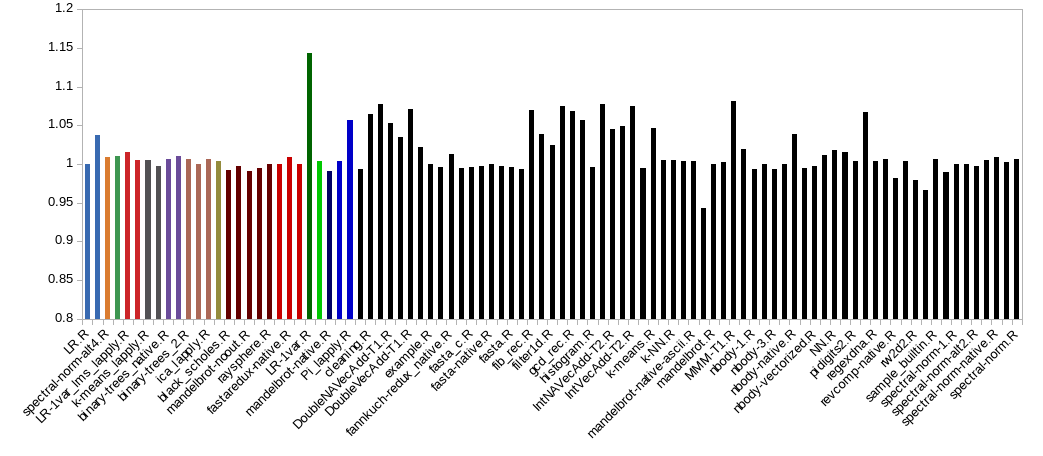
\includegraphics[width=\textwidth]{eval.png}
  \caption{Speedup of an artificial GC parameter change. The black class are the ones classified as noisy or non correlated.}
  \label{fig:eval}
\end{figure}

The relative speedup of this GC tuning is shown in \autoref{fig:eval}.
As an explanation for our result we would like to point out the blue class, left of the big black cluster.
There are two benchmarks with roughly 10\% difference in runtime, but in the same class.
As a matter of fact, they represent cluster 5 from \autoref{fig:c5}.
It seems, even with the high number of $k$, we still end up clustering very different benchmarks into similar categories.

In conclusion we believe that most benchmarks exhibit unique or unpredictable behavior.
Even for benchmarks with similar responses, small differences in the \emph{slow}, \emph{fast} boundary can have big effects in practice.
Therefore, we think it is mostly not the case, that one benchmark can subsume another one.
Based on those findings we do not recommend retiring or skipping benchmarks, and conclude that more work is necessary to accurately predict the effects of GC heuristics changes.

\bibliography{project-R-gc}

\section{Appendix}

Identified Clusters:

{\small
\begin{description}
\item [Not] correlated to GC parameters
\begin{itemize}
\item binary-trees.R, 
\item cleaning.R, 
\item crt.R, 
\item DoubleNAVecAdd-T1.R, 
\item DoubleNAVecAdd-T2.R, 
\item DoubleVecAdd-T2.R, 
\item example.R, 
\item fannkuch-redux\_native.R, 
\item fasta-2.R, 
\item fasta-native2.R, 
\item filter1d.R, 
\item ForLoopAdd.R, 
\item IntNAVecAdd-T1.R, 
\item IntNAVecAdd-T2.R, 
\item IntVecAdd-T1.R, 
\item IntVecAdd-T2.R, 
\item k-means.R, 
\item k-NN\_lapply.R, 
\item k-NN.R, 
\item mandelbrot-noout-native.R, 
\item mandelbrot.R, 
\item MMM-T3.R, 
\item nbody-1.R, 
\item nbody-2.R, 
\item nbody-3.R, 
\item nbody-native.R, 
\item nbody-native2.R, 
\item prime.R, 
\item regexdna.R, 
\item revcomp-1.R, 
\item revcomp-native.R, 
\item rw2d2.R, 
\item rw2d3.R, 
\item sample\_builtin.R, 
\item sample.R, 
\item spectral-norm-1.R, 
\item spectral-norm-alt.R, 
\item spectral-norm-math.R, 
\item spectral-norm-native.R, 
\item spectral-norm.R, 
\end{itemize}

\item[Weak] or very noisy correlation
\begin{itemize}
\item DoubleVecAdd-T1.R, 
\item fannkuch-redux\_2.R, 
\item fannkuch-redux.R, 
\item fasta\_c.R, 
\item fasta-native.R, 
\item fasta.R, 
\item fastaredux.R, 
\item fib\_rec.R, 
\item fib.R, 
\item gcd\_rec.R, 
\item gcd.R, 
\item histogram.R, 
\item k-means-1D.R, 
\item LR\_lms\_lapply.R, 
\item mandelbrot-native-ascii.R, 
\item meteor-contest.R, 
\item MMM-T1.R, 
\item nbody-vectorized.R, 
\item NN\_lapply.R, 
\item NN.R, 
\item pidigits.R, 
\item pidigits2.R, 
\item rw2d1.R, 
\item spectral-norm-alt2.R, 
\item spectral-norm-vectorized.R, 
\end{itemize}

\item[Cluster 1] with
\begin{itemize}
\item LR.R, 
\item MMM-T2.R
\end{itemize}

\item[Cluster 2] with
 \begin{itemize}
\item spectral-norm-alt4.R
 \end{itemize}

\item[Cluster 3] with
 \begin{itemize}
\item LR-1var\_lms\_vec.R
 \end{itemize}

\item[Cluster 4] with
 \begin{itemize}
\item LR-1var\_lms\_lapply.R, 
\item spectral-norm-alt3.R
 \end{itemize}

\item[Cluster 5] with
 \begin{itemize}
\item k-means\_lapply.R, 
\item k-means-1D\_lapply.R
 \end{itemize}

\item[Cluster 6] with
 \begin{itemize}
\item binary-trees\_native.R, 
\item smv.R
 \end{itemize}

\item[Cluster 7] with
 \begin{itemize}
\item binary-trees\_2.R, 
\item binary-trees\_list.R, 
\item ica\_lapply.R
 \end{itemize}

\item[Cluster 8] with
 \begin{itemize}
\item smv\_builtin.R
 \end{itemize}

\item[Cluster 9] with
 \begin{itemize}
\item black\_scholes.R, 
\item mandelbrot-ascii.R, 
\item mandelbrot-noout.R, 
\item mandelbrot1.R, 
\item raysphere.R
 \end{itemize}

\item[Cluster 10] with
 \begin{itemize}
\item fasta-3.R, 
\item fastaredux-native.R, 
\item nbody.R
 \end{itemize}

\item[Cluster 11] with
 \begin{itemize}
\item LR-1var.R
 \end{itemize}

\item[Cluster 12] with
 \begin{itemize}
\item LR\_ols\_lapply.R
 \end{itemize}

\item[Cluster 13] with
 \begin{itemize}
\item mandelbrot-native.R
 \end{itemize}

\item[Cluster 14] with
 \begin{itemize}
\item LR-1var\_ols\_lapply.R, 
\item Pi\_lapply.R
 \end{itemize}
\end{description}
}


\end{document}
